\usepackage{hyperref}\subsection{Einlesen und Verarbeiten von XML-Daten}
\label{subsec:einlesen-und-verarbeiten-von-xml-daten}

Wie bereits im vorherigen Unterkapitel erläutert, beginnt das Einlesen und Verarbeiten mit der Übergabe des Inhaltes aus der
Upload-Seite der Web-Applikation über die Post-Methode.

Die daraus erhaltenen Daten werden in die Funktion \code{upload()} in der Datei \code{route.py} für die Upload-Seite übergeben.
weitergegeben und von der Funktion \code{ingest\_xml()} aus \code{xml\_ingest.py} verarbeitet wird.
Bevor die Daten an \code{ingest\_xml()} übergeben werden, werden diese durch die Funktion \code{parse\_xml\_string()} aus
\code{utils} geparst.
und somit die Struktur der XML-Daten grundlegend überprüft.
Für das Parsen wird die Bibliothek \code{lxml} genutzt.

Die relevanten Daten werden in \code{ingest\_xml()} durch Hilfsfunktionen extrahiert und in Variablen bzw. Listen
vorsortiert und gespeichert.

Die Hilfsfunktionen nutzen hierbei die XPath-Adressierung über die Funktion \code{xpath()} aus der Bibliothek \code{lxml}
bzw. aus dem Modul \code{lxml.etree}, um die relevanten Daten als Listen zurückzugeben.
In Abbildung \ref{} ist zur Veranschaulichung ein Codeabschnitt dargestellt, in den über die Hilfsfunktionen die Variablen
für das Vorsortieren und Speichern befüllt werden.

\begin{figure}[H]
    \centering
    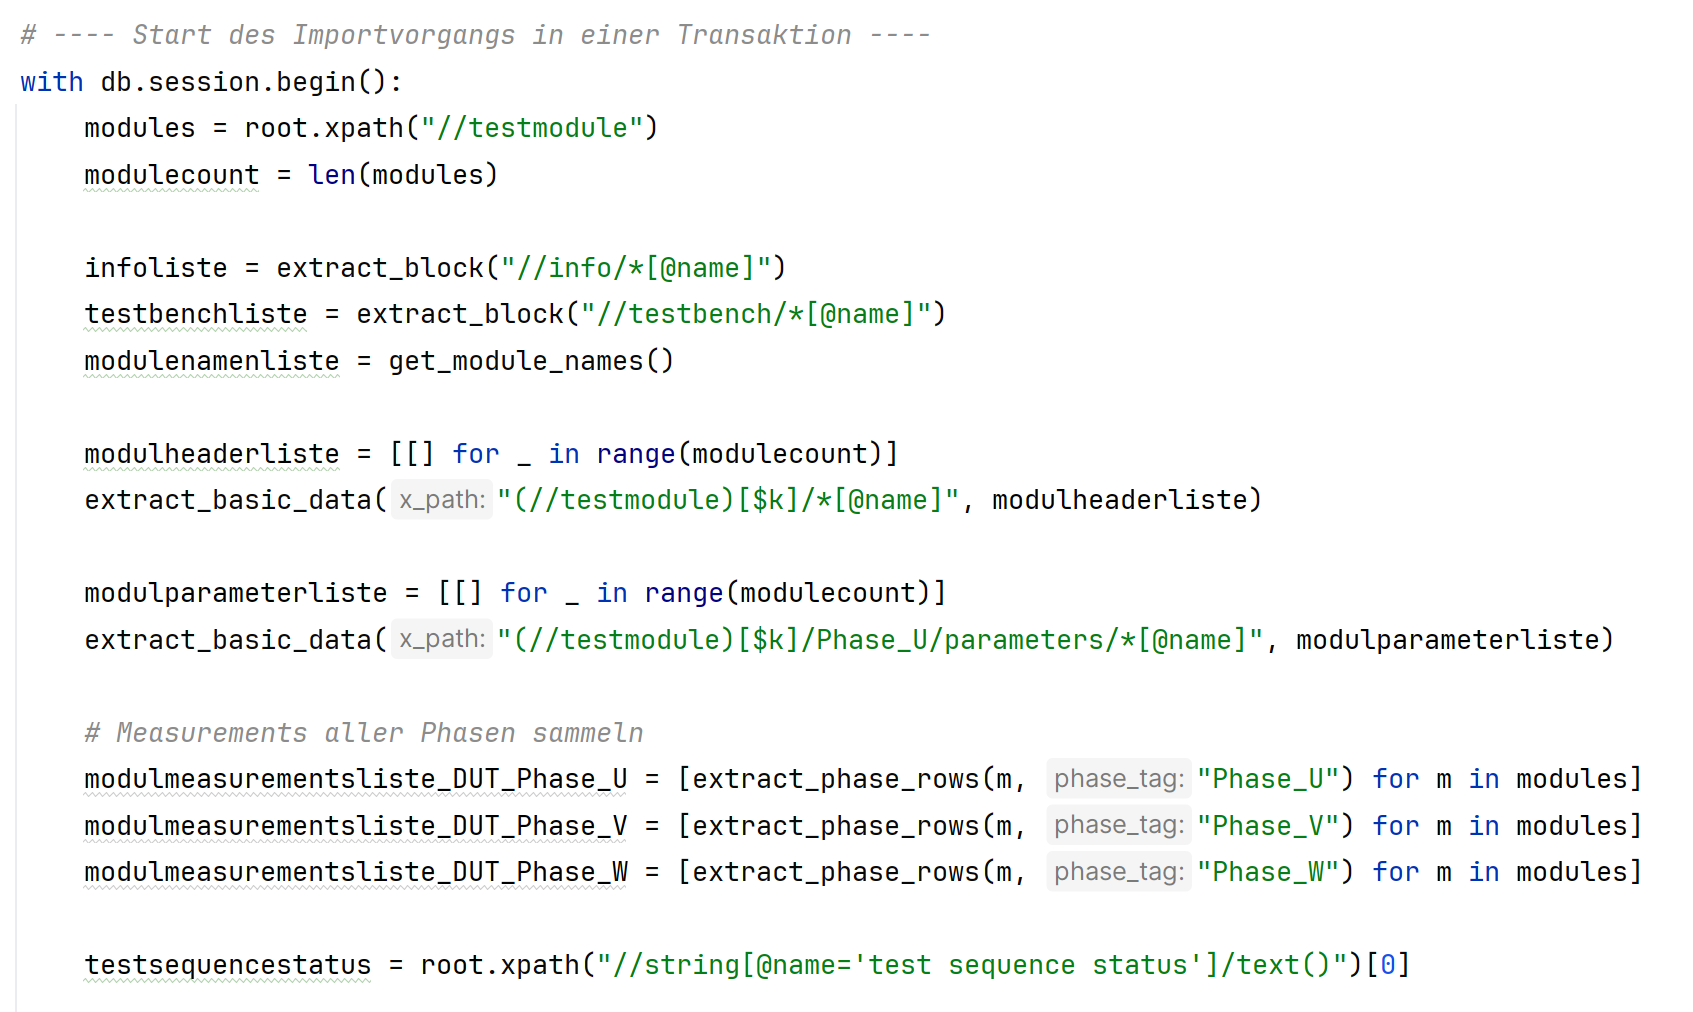
\includegraphics[width=1\textwidth]{Grafiken/5.3 Listen}
    \caption{Grundlegende Ordnerstruktur der Applikations}
    \label{fig: Grundlegende Ordnerstruktur der Applikations}
    {Quelle: Eigene Darstellung mit Microsoft Visio}
\end{figure}

Nach dem Vorsortieren und Speichern werden \ac{ORM}-Objekte für das Überführen der Daten in die Datenbank erstellt.
Mit Hilfe der Suchfunktion \code{get\_value\_by\_name()} werden die Daten anhand der Namen aus den Namen-Attributen gesucht,
die zusammen mit dem Inhalt aus dem XML-Element in Tupeln gespeichert sind.
den Namen-Attribute, welche zusammen mit dem Inhalt aus dem XML-Element in Tupeln gespeichert sind, aus den Listen gesucht.
Der Inhalt wird zurückgegeben, außer wenn der Name nicht gefunden wird.
Dann wird ein Standardwert zurückgegeben.
Dieser Standardwert löst beim Eintragen in die Datenbank bewusst Fehler aus, um Fehler in der Übertragung und der
Verarbeitung der XML-Daten zu erkennen.
Für den Code zu \code{get\_value\_by\_name() siehe Abbildung \ref{}.

\begin{figure}[H]
    \centering
    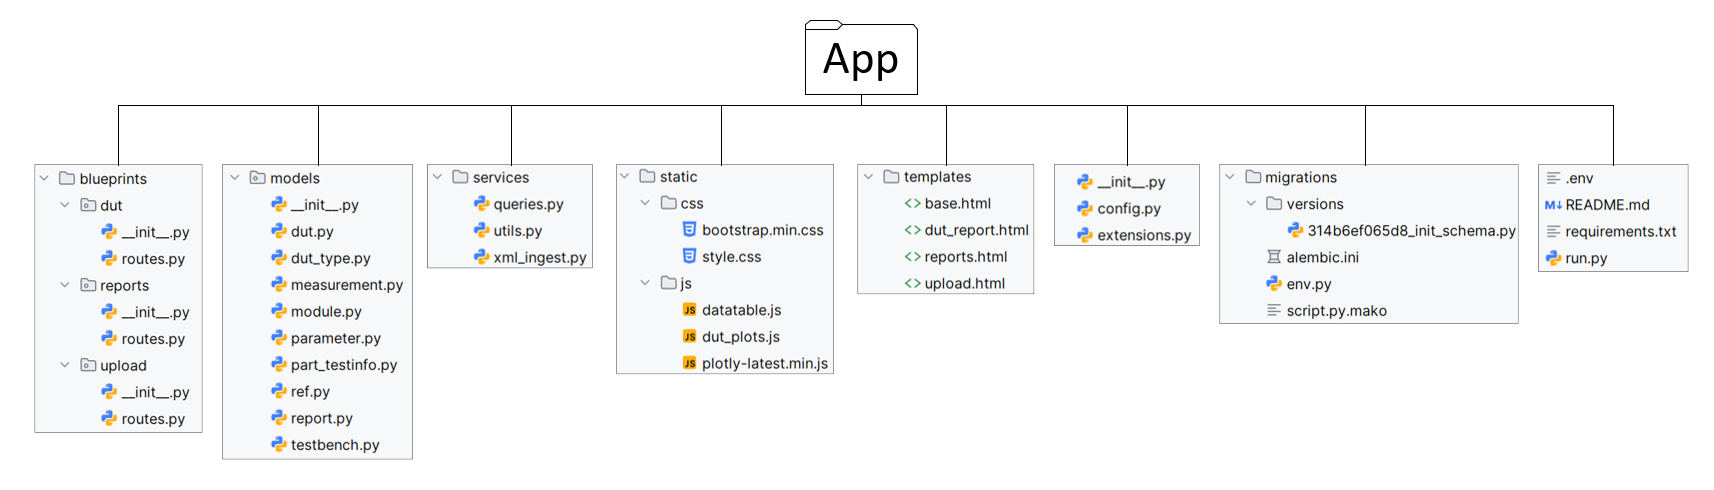
\includegraphics[width=1\textwidth]{Grafiken/Min Ordnerstruktur Projekt}
    \caption{Grundlegende Ordnerstruktur der Applikations}
    \label{fig: Grundlegende Ordnerstruktur der Applikations}
    {Quelle: Eigene Darstellung mit Microsoft Visio}
\end{figure}

Die \ac{ORM}-Objekte werden durch die Funktionen \code{.session.add()} und \code{.session.flush()} schon in die Datenbank geschrieben,
um die automatisch generierten Primärschlüssel der Objekte erhalten zu können.
Die richtige Transaktion der \ac{ORM}-Objekte wird erst am Ende der Funktion \code{ingest\_xml()} ausgeführt, damit nur
vollständig einpflegbare XML-Daten in die Datenbank überführt werden können.
Bei einem Fehler werden alle Transaktionen rückgängig gemacht und die ausstehenden Änderungen gelöscht und es wird ein Fehler zurückgegeben.

Neben dieser Sicherung werden alle vermeintlichen Eintragungen bzw. \ac{ORM}-Objekte noch mal in der Datenbank über
Funktionen \code{execute()} und \code{select()} gesucht.
Wenn das Element bereits in der Datenbank existiert, wird es nicht eingefügt, um Dopplungen zu vermeiden. Ein Codebeispiel für
Die Sicherung ist in Abbildung \ref{} dargestellt.
Die Prüfungen sind in diesem Prototyp nicht identisch und können geringfügige Variationen beinhalten.

\begin{figure}[H]
    \centering
    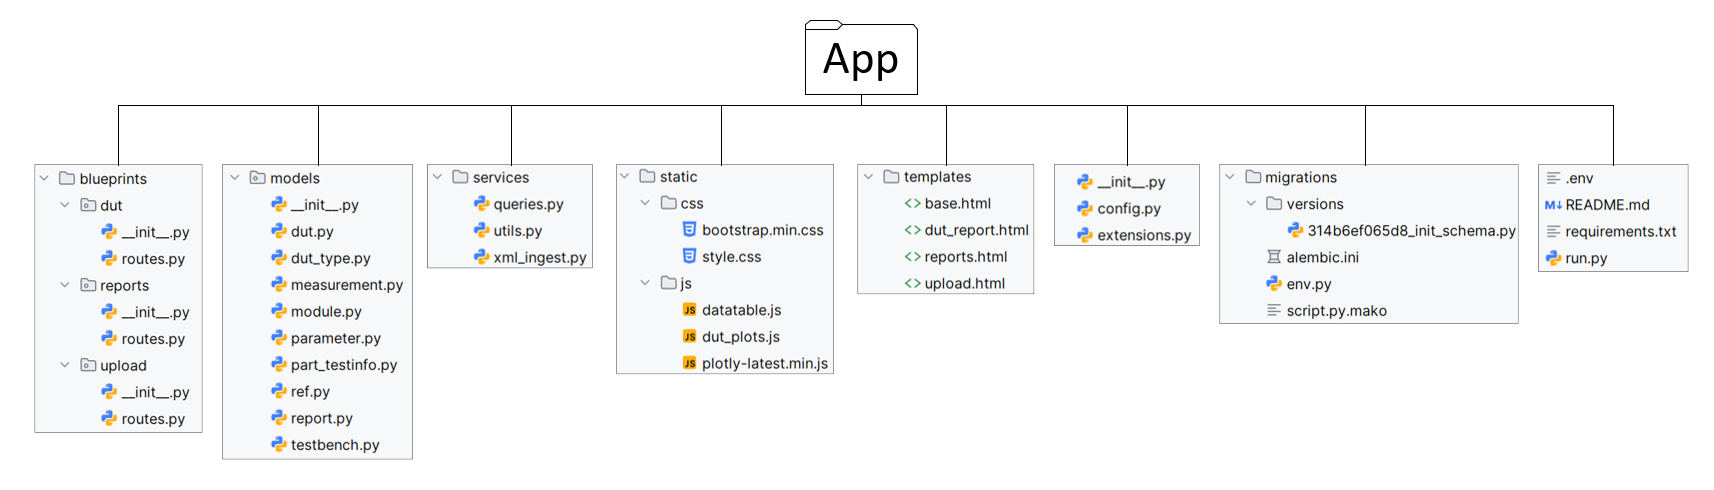
\includegraphics[width=1\textwidth]{Grafiken/Min Ordnerstruktur Projekt}
    \caption{Grundlegende Ordnerstruktur der Applikations}
    \label{fig: Grundlegende Ordnerstruktur der Applikations}
    {Quelle: Eigene Darstellung mit Microsoft Visio}
\end{figure}

Bei einem erfolgreichen Einfügen wird die Report-ID aus dem Eintrag aus der Datenbank an \code{upload()} zurückgegeben.
Diese erstellt dann eine Erfolgsnachricht, welche dann auf der Benutzeroberfläche der Seite ausgegeben wird.
In Abbildung \ref{} ist der Code aus der \code{routes.py}von der Upload-Seite dargestellt.

\begin{figure}[H]
    \centering
    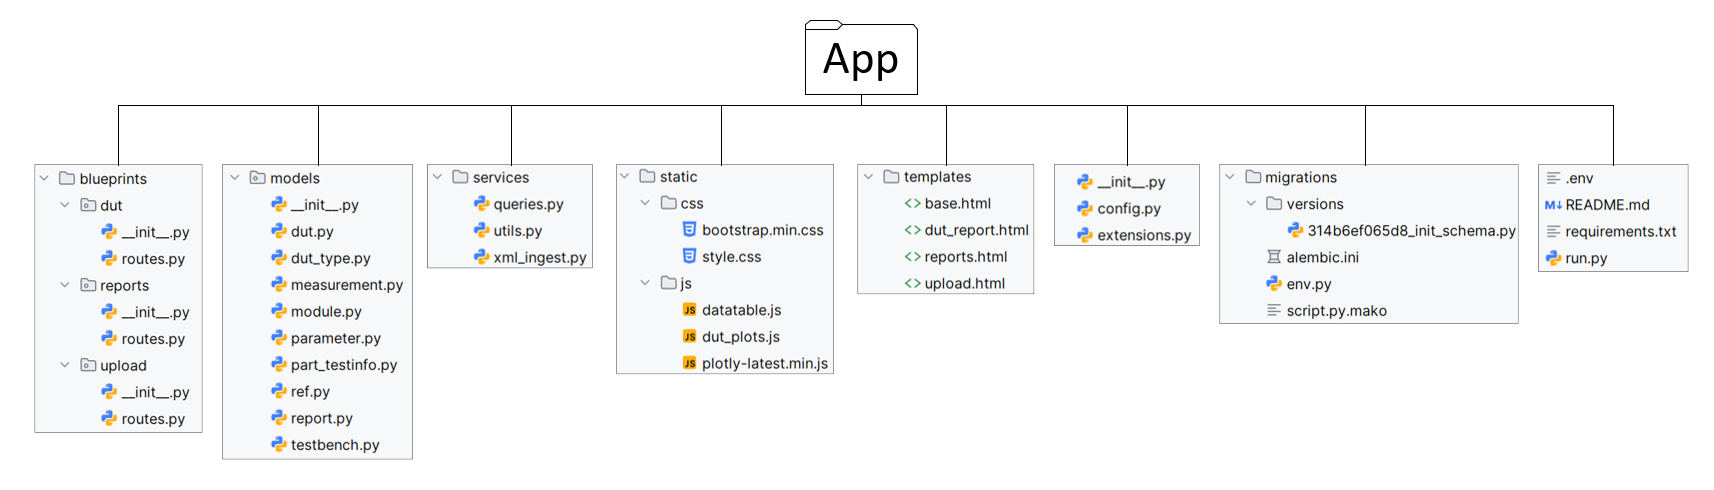
\includegraphics[width=1\textwidth]{Grafiken/Min Ordnerstruktur Projekt}
    \caption{Grundlegende Ordnerstruktur der Applikations}
    \label{fig: Grundlegende Ordnerstruktur der Applikations}
    {Quelle: Eigene Darstellung mit Microsoft Visio}
\end{figure}







